\chapter{Évaluation finale et optimisation du seuil}
\label{chap:evaluation}
\thispagestyle{plain}

\section{Du score probabiliste à la décision clinique}
Un classifieur binaire ne fournit pas directement une décision médicale : il estime d'abord un score ou une probabilité d'appartenance à la classe positive, puis un seuil transforme ce score en prédiction. Avec le seuil conventionnel de 0,50, une observation est déclarée positive si sa probabilité estimée atteint au moins 0,50. Cette convention ne tient pas compte, à elle seule, du déséquilibre de la cible ni du coût asymétrique des erreurs dans un contexte de dépistage.

Lorsque les AVC sont rares et que les faux négatifs sont particulièrement coûteux, un seuil non validé peut laisser trop de cas positifs sous la limite de décision. Le seuil 0,50 n'est cependant pas nécessairement trop élevé pour tous les modèles : son effet dépend de la distribution et de la calibration des probabilités. Il doit donc être choisi empiriquement sur les données d'entraînement, selon un objectif explicite, et non abaissé arbitrairement. Dans l'exécution documentée ici, les seuils optimaux sont même supérieurs à 0,50 ; le seuil de 0,18 donné comme exemple ne correspond pas aux résultats du notebook.

\section{Recherche du seuil sur les probabilités hors pli}
\subsection{Prédictions out-of-fold}
Pour chaque finaliste — régression logistique pondérée, Random Forest pondérée et XGBoost avec \texttt{scale\_pos\_weight} — les probabilités de la classe AVC sont estimées sur le jeu d'entraînement au moyen de \texttt{cross\_val\_predict(method="predict\_proba")}, avec une validation croisée \texttt{StratifiedKFold} à cinq plis. Ainsi, chaque observation d'entraînement reçoit une probabilité produite par un modèle qui n'a pas été ajusté sur cette observation. Le seuil est donc déterminé à partir de prédictions hors pli, plutôt qu'à partir des probabilités d'ajustement du modèle entraîné sur toutes les données, ce qui limite un seuil artificiellement optimiste.

À partir des probabilités hors pli, la courbe précision-rappel fournit, pour chaque seuil candidat, une précision \(P\) et un rappel \(R\). Le score \(F_\beta\) est une moyenne harmonique pondérée de ces deux mesures. Le choix \(\beta=2\) donne davantage de poids au rappel qu'à la précision :
\[
F_2 = (1+\beta^2)\frac{P\,R}{\beta^2P+R}
    = \frac{5\,P\,R}{4P+R}.
\]
Le seuil retenu pour chaque modèle est celui qui maximise le \(F_2\) calculé sur ces probabilités hors pli. Les divisions par zéro sont traitées dans le calcul numérique afin que les seuils sans prédictions positives ne provoquent pas d'échec. La figure~\ref{fig:threshold-f2} présente les courbes obtenues et les seuils maximisants.

\begin{figure}[H]
    \centering
    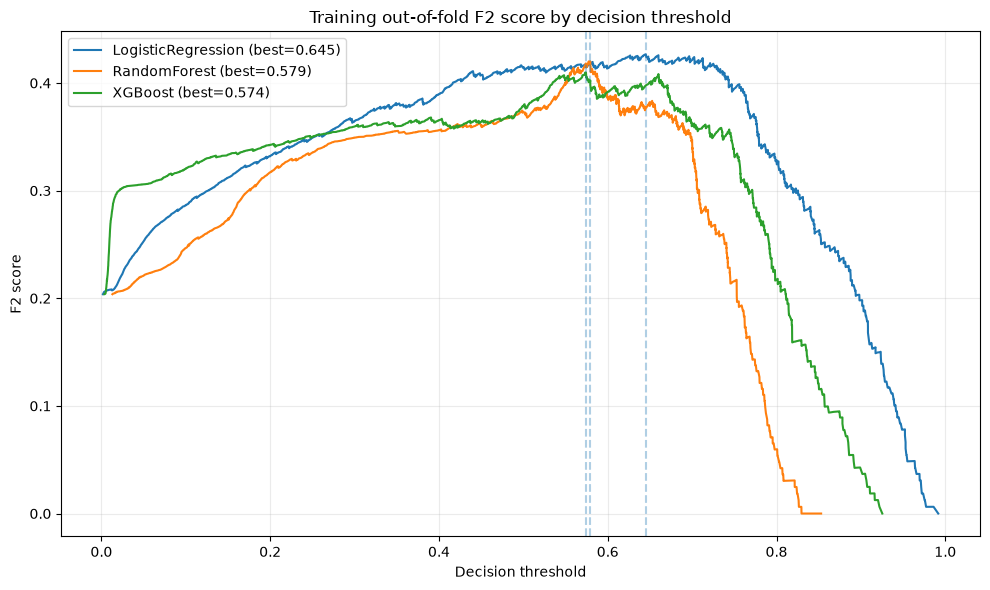
\includegraphics[width=0.82\textwidth]{figures/04_threshold_f2.png}
    \caption{Score \(F_2\) selon le seuil, calculé sur les probabilités out-of-fold du jeu d'entraînement. Les lignes verticales indiquent les seuils maximisant le \(F_2\) pour chaque modèle.}
    \label{fig:threshold-f2}
\end{figure}

Les seuils et scores hors pli effectivement obtenus sont synthétisés au tableau~\ref{tab:threshold-oof}. Ces valeurs sont des résultats d'optimisation sur le train, et non des mesures obtenues sur le test.

\begin{table}[H]
    \centering
    \caption{Optimisation des seuils sur les prédictions out-of-fold du train}
    \label{tab:threshold-oof}
    \small
    \begin{tabular}{@{}lrrr@{}}
        \toprule
        \textbf{Modèle} & \textbf{Seuil optimal} & \textbf{\(F_2\) OOF} & \textbf{Rappel OOF}\\
        \midrule
        LogisticRegression & 0,645058 & 0,427 & 0,678\\
        RandomForest & 0,579257 & 0,420 & 0,769\\
        XGBoost & 0,574196 & 0,410 & 0,729\\
        \bottomrule
    \end{tabular}
\end{table}

\subsection{Plancher de spécificité et compromis d'alertes}
Maximiser le rappel sans contrainte peut conduire à classer un grand nombre de patients non AVC comme positifs. La spécificité mesure la proportion de négatifs correctement rejetés :
\[
\operatorname{Specificite} = \frac{TN}{TN+FP},
\]
où \(TN\) et \(FP\) désignent respectivement les vrais négatifs et les faux positifs. Pour rendre explicite le compromis avec la charge d'alertes, un plancher de spécificité de 0,70 a été fixé avant l'examen des résultats du test. Il limite à 30\,\% au plus le taux de faux positifs parmi les sujets sains, selon le critère retenu par le protocole.

Ce seuil de 0,70 est une contrainte opérationnelle de cette étude, et non une norme clinique universelle. Il sert à éviter une stratégie qui maximiserait le rappel au prix d'un nombre d'alertes potentiellement ingérable, mais sa pertinence doit être confirmée avec les professionnels de santé et le contexte réel de déploiement. La sélection du modèle est effectuée exclusivement à partir des métriques OOF : parmi les candidats dont la spécificité OOF atteint le plancher, la règle retient celui qui présente le rappel OOF le plus élevé, avec le \(F_2\) et la spécificité comme critères de départage.

\section{Évaluation finale sur le test indépendant}
Une fois les seuils déterminés et la règle de sélection arrêtée sur le train, les modèles ajustés sur l'ensemble du train calculent les probabilités du test. Les prédictions sont obtenues en comparant chaque probabilité au seuil déjà figé. Le jeu de test n'intervient ni dans le calcul des seuils ni dans le choix du modèle ; il est réservé à cette évaluation finale.

Le tableau~\ref{tab:resultats-test-seuils} présente les métriques du test, composé de 1\,022 observations : 972 sujets sains et 50 cas AVC. Les valeurs illustrent l'amélioration de la détection positive tout en maintenant, pour chacun des trois seuils testés, une spécificité supérieure au plancher fixé.

\begin{table}[H]
    \centering
    \caption{Résultats sur le jeu de test avec les seuils optimisés sur le train}
    \label{tab:resultats-test-seuils}
    \small
    \begin{tabular}{@{}lrrrrrr@{}}
        \toprule
        \textbf{Modèle} & \textbf{Seuil} & \textbf{Rappel} & \textbf{Précision} & \textbf{Spécificité} & \textbf{FN} & \textbf{FP}\\
        \midrule
        LogisticRegression & 0,645058 & 0,72 & 0,178 & 0,829 & 14 & 166\\
        RandomForest & 0,579257 & 0,80 & 0,150 & 0,766 & 10 & 227\\
        XGBoost & 0,574196 & 0,76 & 0,162 & 0,798 & 12 & 196\\
        \bottomrule
    \end{tabular}
\end{table}

La figure~\ref{fig:matrices-confusion} montre les matrices de confusion correspondantes. Les cellules inférieures gauches représentent les AVC classés à tort comme sains, c'est-à-dire les faux négatifs. Sur ces 50 cas positifs, la Random Forest en manque 10, XGBoost 12 et la régression logistique 14. La Random Forest atteint ainsi le rappel test le plus élevé, 0,80, tout en conservant une spécificité de 0,766, supérieure au plancher. Ces résultats ne suppriment toutefois pas le compromis : sa précision de 0,150 et ses 227 faux positifs sur 972 sujets sains indiquent une charge d'alertes encore importante, à examiner avant toute utilisation clinique.

\begin{figure}[H]
    \centering
    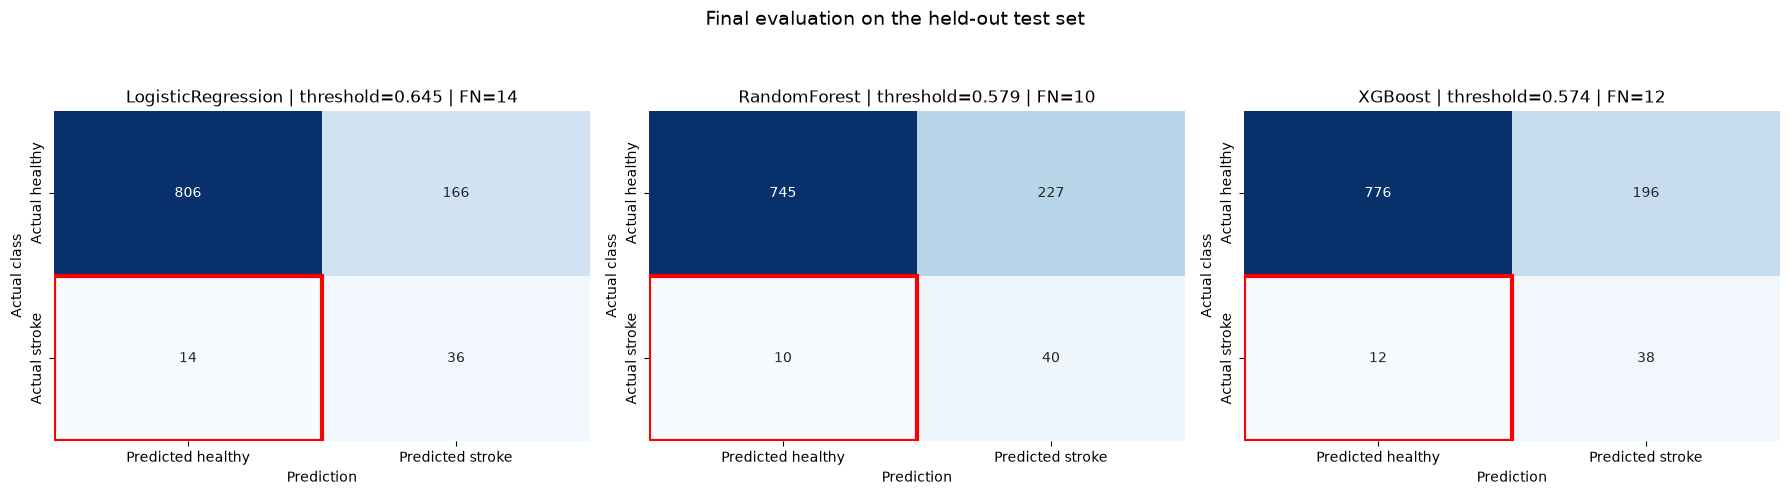
\includegraphics[width=\textwidth]{figures/05_confusion_matrices.png}
    \caption{Matrices de confusion sur le test pour les trois modèles et leurs seuils optimisés sur le train. Les faux négatifs, situés en bas à gauche, sont encadrés en rouge.}
    \label{fig:matrices-confusion}
\end{figure}

\section{Sélection du modèle champion et export}
Le modèle champion est choisi sans consulter les scores du test : la règle appliquée sélectionne le modèle au rappel OOF le plus élevé parmi ceux satisfaisant le plancher de spécificité. Selon l'exécution du notebook, le modèle retenu est la \textbf{Random Forest}, avec un rappel OOF de 0,769 et une spécificité OOF de 0,776 au seuil correspondant. Son rappel test de 0,80 confirme ensuite, à titre d'évaluation indépendante, le résultat de cette sélection.

Le modèle réentraîné sur l'intégralité du jeu d'entraînement et ses métadonnées sont exportés aux emplacements suivants :
\begin{itemize}
    \item Modèle : \path{../data/processed/final_model.joblib} ;
    \item Métadonnées : \path{../data/processed/model_metadata.json}.
\end{itemize}
Les métadonnées conservent notamment le nom du modèle, la règle de sélection, la spécificité minimale et le seuil numérique exact. Pour le modèle exporté, ce seuil vaut :
\[
\texttt{decision\_threshold} = 0.5792571442648802.
\]
La future API FastAPI devra charger le modèle et appliquer cette valeur exacte à la probabilité de la classe AVC, selon la règle \(p \geq \texttt{decision\_threshold}\). Remplacer ce seuil par 0,50 — ou par la valeur d'exemple 0,18 — modifierait le comportement validé et les compromis mesurés. L'ordre des caractéristiques enregistré dans les métadonnées doit également être respecté lors de la construction de l'entrée du modèle.

\section{Portée et limites de l'évaluation}
Cette évaluation confirme la faisabilité d'un réglage de seuil orienté vers le rappel tout en imposant une contrainte explicite sur la spécificité. Elle ne constitue pas une validation clinique du système : la faible précision observée, la variabilité liée à un nombre limité de cas AVC dans le test et les conséquences opérationnelles des faux positifs requièrent une étude complémentaire. Avant tout déploiement, il faudra notamment valider le pipeline complet sur des données externes, vérifier la calibration des probabilités, suivre les performances selon les sous-groupes pertinents et faire approuver le seuil par les responsables cliniques.
